\begin{tikzpicture}[
			window/.style={draw=red, dashed, line width=0.6pt},
			condtag/.style={draw=none, fill=none, inner sep=1.7pt,
					font=\scriptsize, text=black, align=center,
					text height=1.5ex, text depth=0.25ex}
		]
		\node[inner sep=0] (wave) {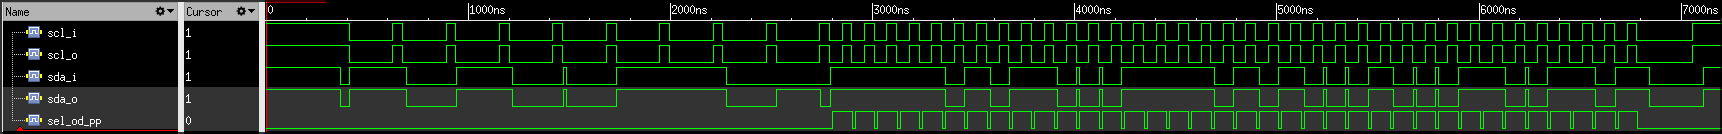
\includegraphics[width=\textwidth]{i3c_write/i3c_write.png}};
		% Toa do chuan hoa theo anh: (0,0) la goc trai duoi, (1,1) la goc phai tren.
		\begin{scope}[shift={(wave.south west)},
				x={($(wave.south east)-(wave.south west)$)},
				y={($(wave.north west)-(wave.south west)$)}]
			\draw[window] (0.185,-0.14) rectangle (0.215,1.14);
			\draw[window] (0.220,-0.14) rectangle (0.4835,1.14);
			\draw[window] (0.4885,-0.14) rectangle (0.963,1.14);
			\draw[window] (0.968,-0.14) rectangle (1.000,1.14);
			\node[condtag, anchor=south] at (0.200,1.16) {S};
			\node[condtag, anchor=south] at (0.35175,1.16) {Address Phase};
			\node[condtag, anchor=north] at (0.35175,-0.16) {0x53, RnW = Write};
			\node[condtag, anchor=south] at (0.72575,1.16) {Data Phase};
			\node[condtag, anchor=north] at (0.72575,-0.16) {FA 8F A2 66};
			\node[condtag, anchor=south] at (0.984,1.16) {P};
		\end{scope}
	\end{tikzpicture}
